% --- ZeRO and FSDP ---
\begin{frame}{ZeRO: Data Parallelism Without the Redundancy}
  \begin{itemize}\scriptsize\itemsep0.05em
    \item[\textcolor{red}{$\blacktriangleright$}] The insight is almost embarrassingly simple. In DDP, rank $r$ stores all $16\Psi$ bytes but, at the moment of the optimizer step, only \emph{uses} $1/d$ of the optimizer states to update $1/d$ of the parameters. The rest is idle storage.
    \item[\textcolor{red}{$\blacktriangleright$}] \textbf{ZeRO} (Zero Redundancy Optimizer) partitions the model states across the $d$ data-parallel ranks instead of replicating them, and communicates the missing pieces \emph{just in time}. The programming model stays data-parallel; only the storage changes.
  \end{itemize}
  \vspace{0.06em}
  \centering
  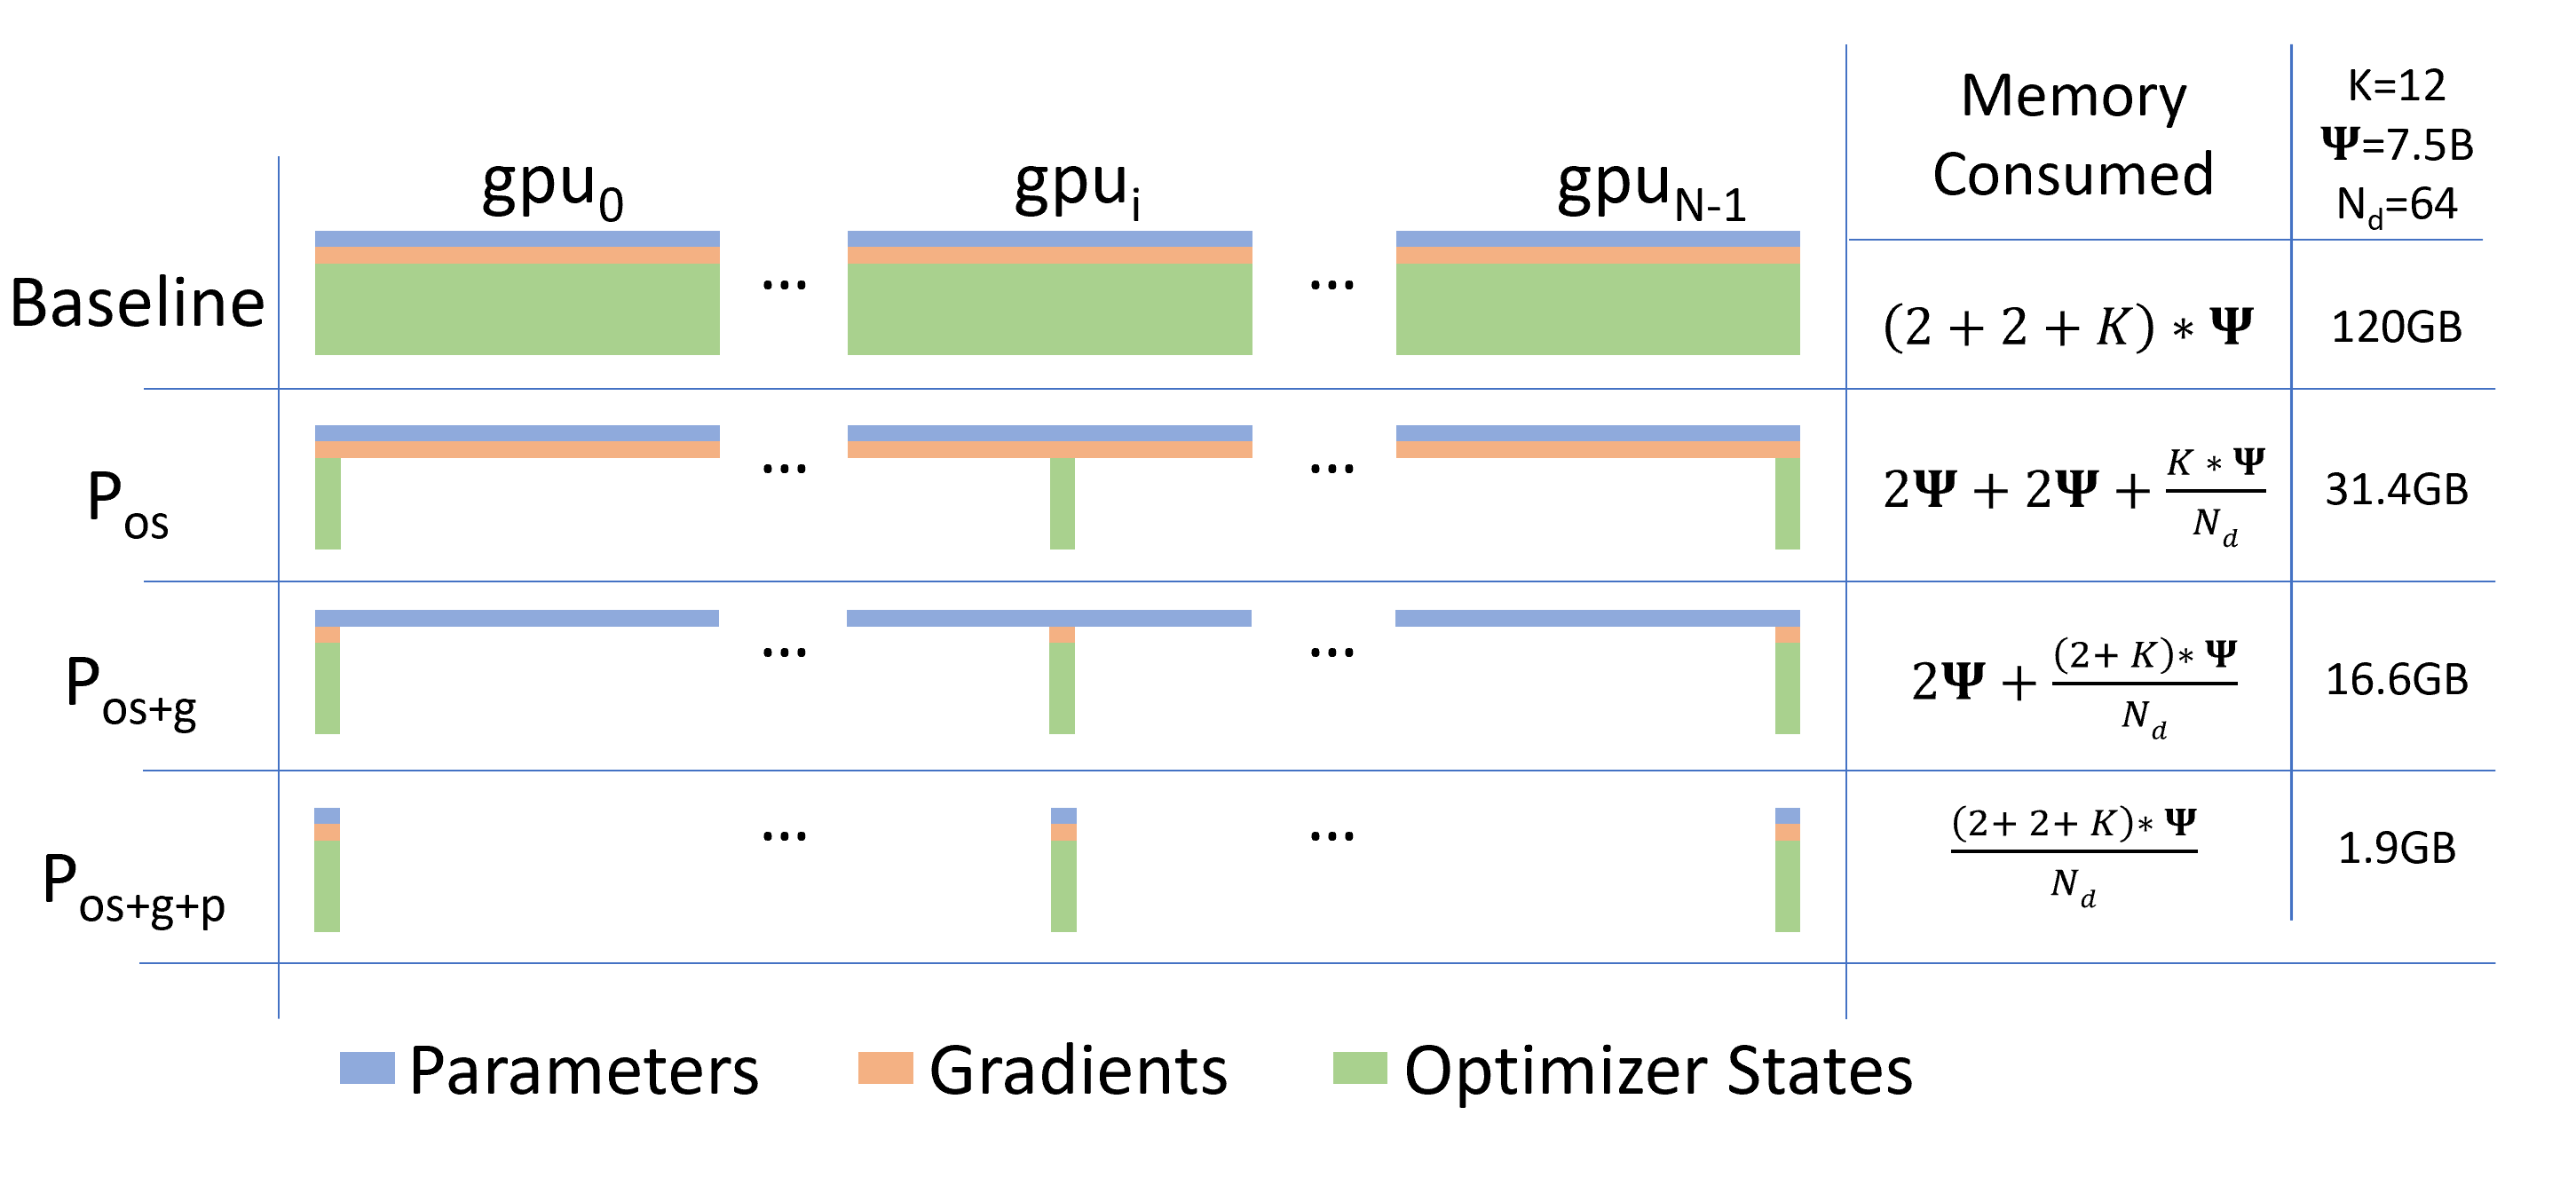
\includegraphics[width=0.86\textwidth,height=0.52\textheight,keepaspectratio]{images/distributed-training/zero_fig1_memory_consumption_stages.png}\\[0.25em]
  {\scriptsize Per-device memory of the model states under the three ZeRO-DP stages, for $\Psi = 7.5$B, $N_d = 64$, $K = 12$. Rajbhandari et al., ``ZeRO: Memory Optimizations Toward Training Trillion Parameter Models,'' \href{https://arxiv.org/abs/1910.02054v3}{arXiv:1910.02054v3}, Figure 1.}
\end{frame}

\begin{frame}{The Three Stages}
  \centering
  \footnotesize
  \begin{tabular}{@{}llll@{}}
    \toprule
    \textbf{Stage} & \textbf{What is partitioned} & \textbf{Bytes per rank} & \textbf{Communication} \\
    \midrule
    Baseline DDP           & nothing                              & $16\Psi$                  & $2\Psi$ (all-reduce) \\
    ZeRO-1 ($P_{os}$)      & optimizer states                     & $4\Psi + 12\Psi/d$        & $2\Psi$ (unchanged) \\
    ZeRO-2 ($P_{os+g}$)    & $+$ gradients                        & $2\Psi + 14\Psi/d$        & $2\Psi$ (unchanged) \\
    ZeRO-3 ($P_{os+g+p}$)  & $+$ parameters                       & $16\Psi/d$                & $3\Psi$ \ ($1.5\times$) \\
    \bottomrule
  \end{tabular}
  \vspace{0.7em}
  \begin{itemize}\footnotesize\itemsep0.25em
    \item[\textcolor{red}{$\blacktriangleright$}] The reductions in the limit of large $d$ are \textbf{4$\times$}, \textbf{8$\times$}, and \textbf{$d\times$}. Only stage 3 removes the constant term, which is why only stage 3 lets model size grow with the cluster.
    \item[\textcolor{red}{$\blacktriangleright$}] \textbf{Stages 1 and 2 are free.} Standard DDP already implements the all-reduce as a reduce-scatter followed by an all-gather; ZeRO simply keeps the intermediate partitioned result instead of throwing it away. Same $2\Psi$ of traffic, less memory.
    \item[\textcolor{red}{$\blacktriangleright$}] \textbf{Stage 3 costs 50\% more traffic.} Parameters must be all-gathered once for the forward pass and once again for the backward pass, on top of the gradient reduce-scatter: $\Psi + \Psi + \Psi = 3\Psi$.
    \item[\textcolor{red}{$\blacktriangleright$}] All communication volumes are counted in \emph{elements}; multiply by 2 for \texttt{bf16} bytes.
  \end{itemize}
\end{frame}

\begin{frame}{ZeRO in Numbers}
  \begin{itemize}\footnotesize\itemsep0.3em
    \item[\textcolor{red}{$\blacktriangleright$}] \textbf{A 7B model on one node of 8$\times$80\,GB.} Model states are $16\Psi = 112$\,GB, so DDP is out of the question. Per GPU:
  \end{itemize}
  \vspace{0.2em}
  \centering
  \footnotesize
  \begin{tabular}{@{}lrrl@{}}
    \toprule
    \textbf{Configuration} & \textbf{Model states / GPU} & \textbf{Free for activations} & \textbf{Verdict} \\
    \midrule
    DDP                    & $112$\,GB                              & ---              & out of memory \\
    ZeRO-1, $d = 8$        & $4\Psi + 12\Psi/8 = 28 + 10.5 = 38.5$\,GB & $41.5$\,GB    & fits \\
    ZeRO-2, $d = 8$        & $2\Psi + 14\Psi/8 = 14 + 12.25 = 26.3$\,GB & $53.7$\,GB   & fits, larger batch \\
    ZeRO-3, $d = 8$        & $16\Psi/8 = 14$\,GB                    & $66$\,GB         & fits, largest batch \\
    \bottomrule
  \end{tabular}
  \vspace{0.7em}
  \begin{itemize}\footnotesize\itemsep0.25em
    \item[\textcolor{red}{$\blacktriangleright$}] \textbf{A 70B model.} Model states are $1.12$\,TB. On 8 GPUs, ZeRO-3 needs $1120/8 = 140$\,GB per GPU --- still impossible. On 16 it is $70$\,GB, which leaves nothing for activations. \textbf{32 GPUs} gives $35$\,GB per GPU and is the first configuration that actually works.
    \item[\textcolor{red}{$\blacktriangleright$}] This arithmetic is the single most useful thing in this lecture: before you launch a job, divide $16\Psi$ by your GPU count and see whether the answer leaves room to breathe.
    \item[\textcolor{red}{$\blacktriangleright$}] \textbf{Offload} extends the ladder downwards. ZeRO-Offload moves optimizer states and the optimizer step to CPU memory and trained \textbf{13B parameters on a single GPU}; ZeRO-Infinity adds NVMe and fine-tunes trillion-parameter models on one DGX-2 node. Both trade PCIe bandwidth for capacity, so they are for ``it must run'' rather than ``it must be fast''.
  \end{itemize}
  \vspace{0.1em}
  {\scriptsize Ren et al., \href{https://arxiv.org/abs/2101.06840v1}{arXiv:2101.06840v1}; Rajbhandari et al., \href{https://arxiv.org/abs/2104.07857v1}{arXiv:2104.07857v1}.}
\end{frame}

\begin{frame}{PyTorch FSDP: the Native Implementation}
  \begin{itemize}\footnotesize\itemsep0.3em
    \item[\textcolor{red}{$\blacktriangleright$}] \textbf{Fully Sharded Data Parallel} is PyTorch's in-tree realisation of the ZeRO-3 idea. The model is decomposed into \textbf{FSDP units}; each unit $i$'s $\psi_i$ parameters are flattened and sharded across $F$ ranks.
    \item[\textcolor{red}{$\blacktriangleright$}] The runtime loop, per unit: \textbf{all-gather} the full parameters just before the unit runs, compute, \textbf{free} the peer shards immediately afterwards, and \textbf{reduce-scatter} the gradients on the way back.
    \item[\textcolor{red}{$\blacktriangleright$}] Peak \emph{parameter} memory is therefore $\sum_i \psi_i / F + \max_i \psi_i$: the sharded whole, plus \emph{one} materialised unit. That $\max_i \psi_i$ term is the entire reason unit granularity matters.
  \end{itemize}
  \vspace{0.2em}
  \centering
  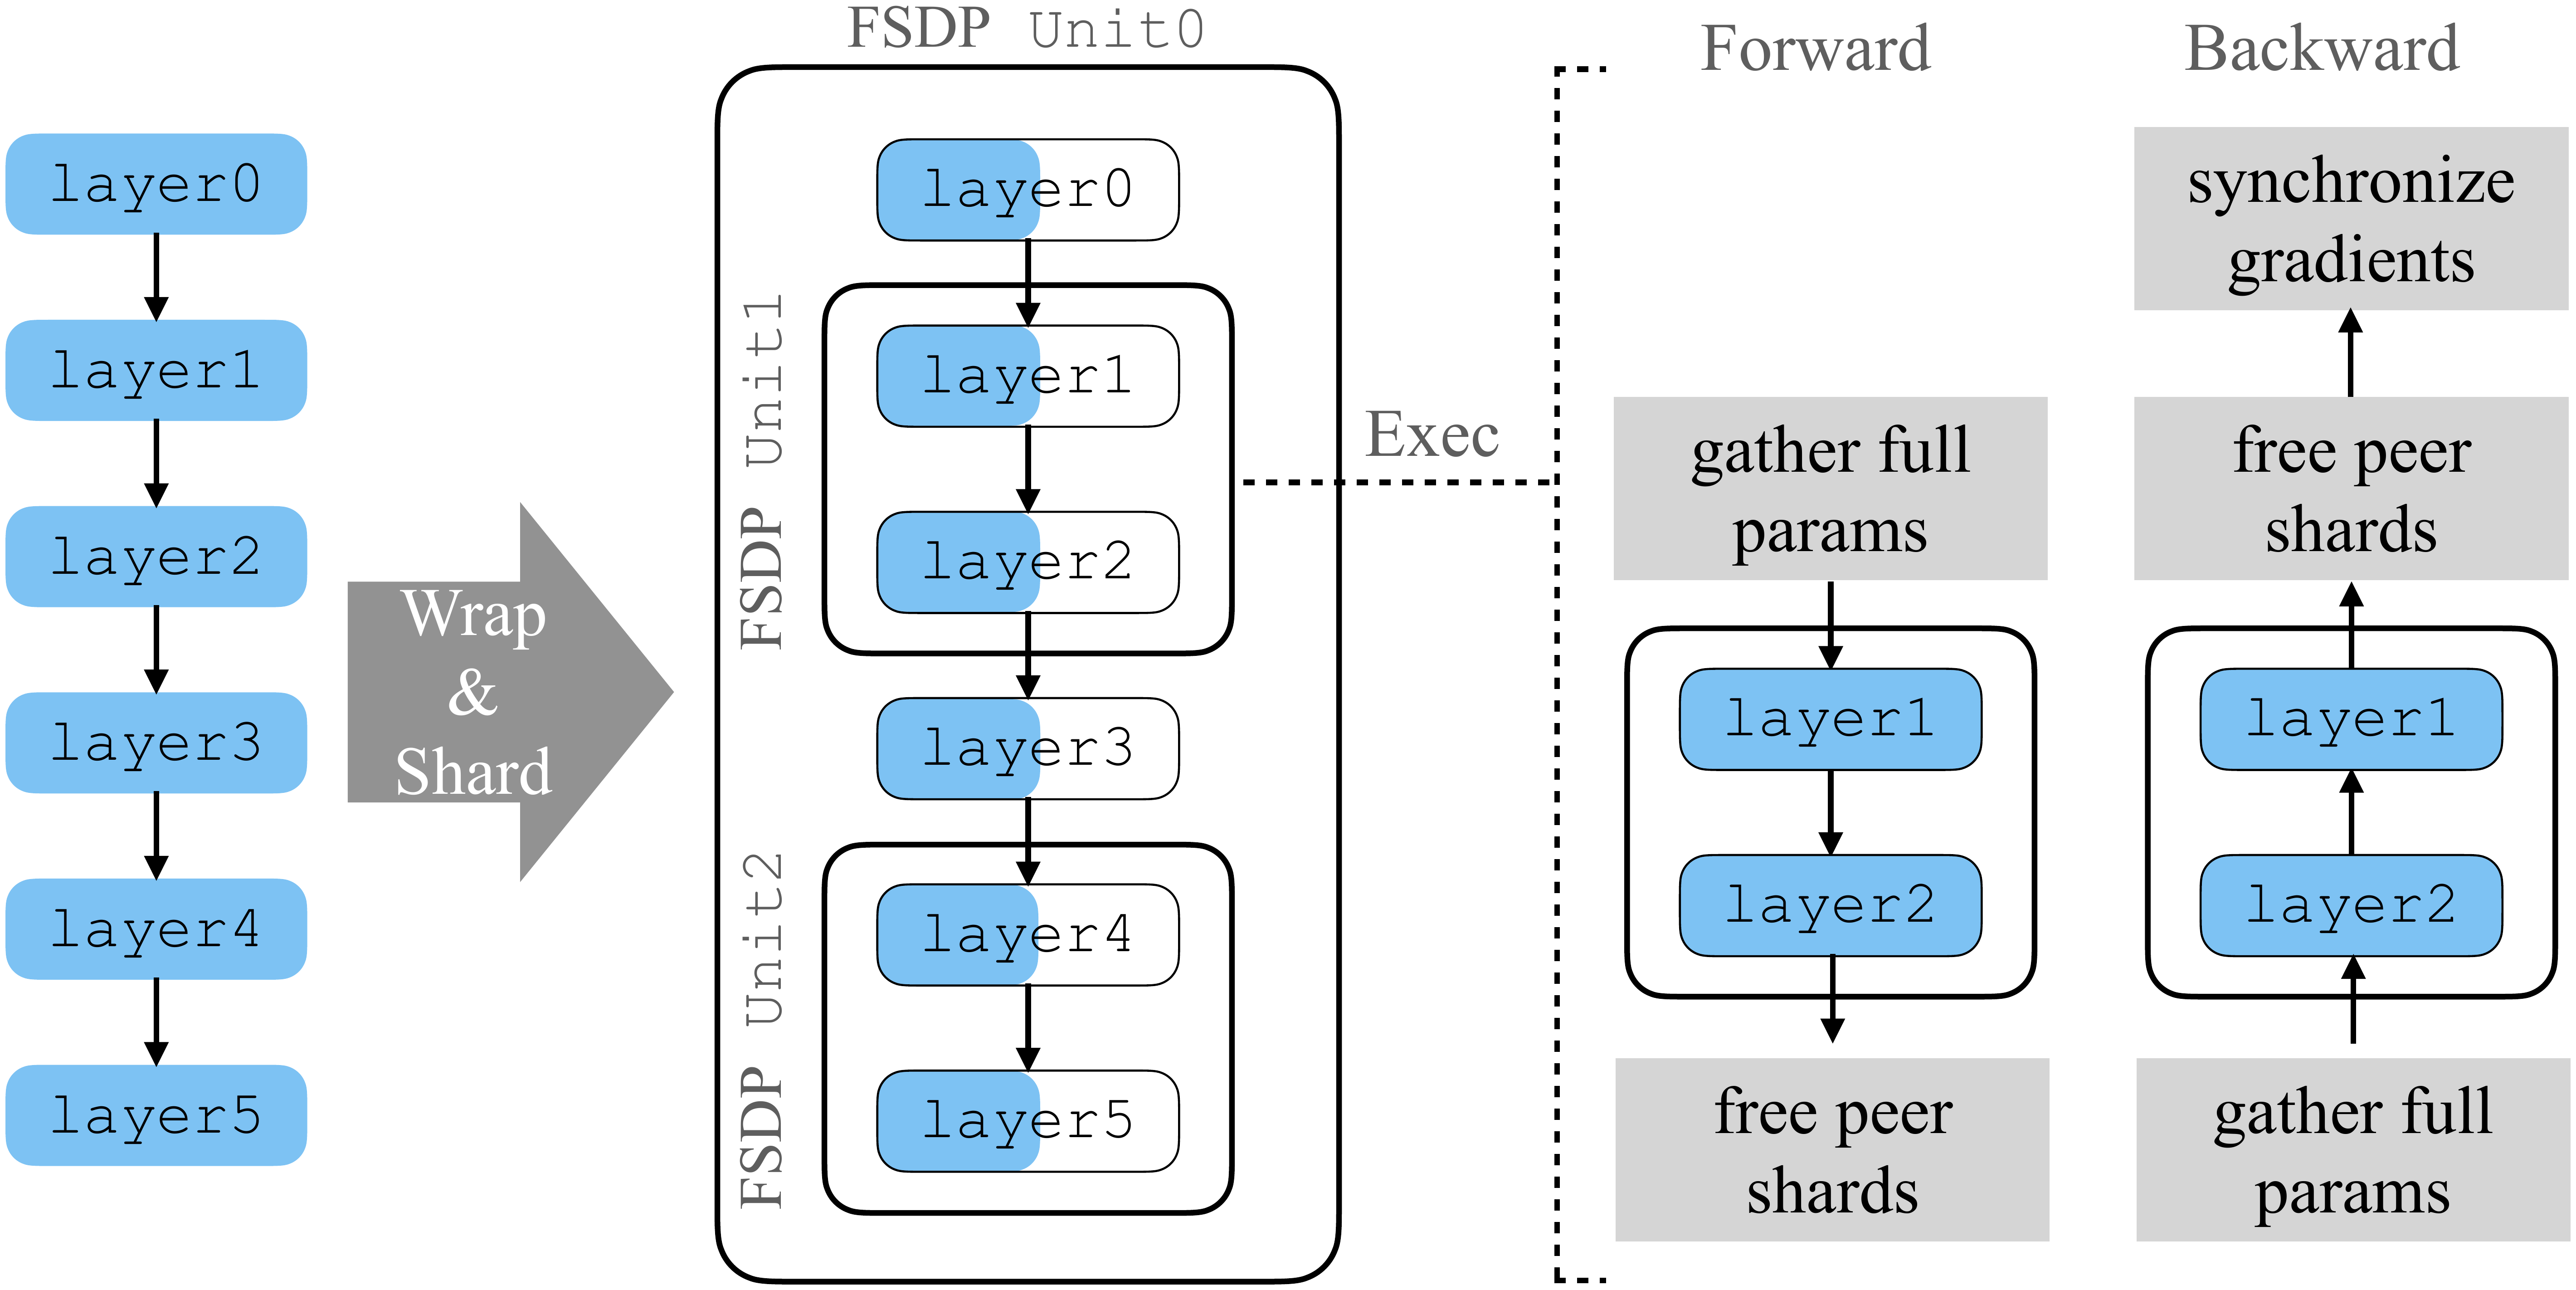
\includegraphics[width=0.88\textwidth,height=0.44\textheight,keepaspectratio]{images/distributed-training/fsdp_fig1_algorithm_overview.png}\\[0.2em]
  {\scriptsize Zhao et al., ``PyTorch FSDP: Experiences on Scaling Fully Sharded Data Parallel,'' VLDB 2023. \href{https://arxiv.org/abs/2304.11277v2}{arXiv:2304.11277v2}, Figure 1.}
\end{frame}

\begin{frame}[allowframebreaks]{Wrapping Policy: the Knob That Decides Everything}
  \begin{itemize}\itemsep0.4em
    \item[\textcolor{red}{$\blacktriangleright$}] The \textbf{auto-wrap policy} decides where unit boundaries fall, and it sets a direct trade-off:
      \begin{itemize}\itemsep0.2em\footnotesize
        \item \textbf{Fine-grained units} (one per transformer block) $\Rightarrow$ small $\max_i \psi_i$, so low peak memory, but many small collectives.
        \item \textbf{Coarse units} (one per model) $\Rightarrow$ few large collectives at peak bandwidth, but the whole model must materialise at once, which defeats the point.
      \end{itemize}
    \item[\textcolor{red}{$\blacktriangleright$}] For transformers the right answer is almost always \textbf{one FSDP unit per transformer block} --- \texttt{transformer\_auto\_wrap\_policy} with the block class, or the model's \texttt{\_no\_split\_modules} in Hugging Face.
    \item[\textcolor{red}{$\blacktriangleright$}] Two further overlaps are worth knowing because they are on by default and occasionally need turning off:
      \begin{itemize}\itemsep0.2em\footnotesize
        \item \textbf{Forward prefetch:} start the all-gather for unit $i+1$ while unit $i$ computes.
        \item \textbf{Backward prefetch:} same idea in reverse, which is where most of FSDP's speed comes from.
      \end{itemize}
    \item[\textcolor{red}{$\blacktriangleright$}] Zhao et al.\ measured all-gather time rising sharply once the message drops below $33$M elements --- concrete evidence for not wrapping every \texttt{nn.Linear} separately.
    \item[\textcolor{red}{$\blacktriangleright$}] Combine FSDP with activation checkpointing at the \emph{same} block boundary. The two are orthogonal: FSDP shards the model states, checkpointing shrinks the activations.
  \end{itemize}
\end{frame}

\begin{frame}{Sharding Strategies}
  \begin{columns}[T,onlytextwidth]
    \column{0.55\textwidth}
      \begin{itemize}\footnotesize\itemsep0.3em
        \item[\textcolor{red}{$\blacktriangleright$}] \texttt{FULL\_SHARD} --- parameters, gradients, and optimizer states all sharded. This is ZeRO-3.
        \item[\textcolor{red}{$\blacktriangleright$}] \texttt{SHARD\_GRAD\_OP} --- gradients and optimizer states sharded; parameters stay gathered between forward and backward. This is ZeRO-2: one fewer all-gather, more memory.
        \item[\textcolor{red}{$\blacktriangleright$}] \texttt{NO\_SHARD} --- plain replication, i.e.\ DDP, useful as a baseline inside the same code path.
        \item[\textcolor{red}{$\blacktriangleright$}] \texttt{HYBRID\_SHARD} --- \emph{shard within a node, replicate across nodes}. The expensive all-gathers stay on NVLink; only a gradient all-reduce crosses the slow inter-node fabric.
        \item[\textcolor{red}{$\blacktriangleright$}] \texttt{CPUOffload(offload\_params=True)} --- park parameters and gradients in host memory and run the optimizer step on the CPU. Last resort; PCIe becomes the bottleneck.
      \end{itemize}
    \column{0.43\textwidth}
      \centering
      \vspace{0.5em}
      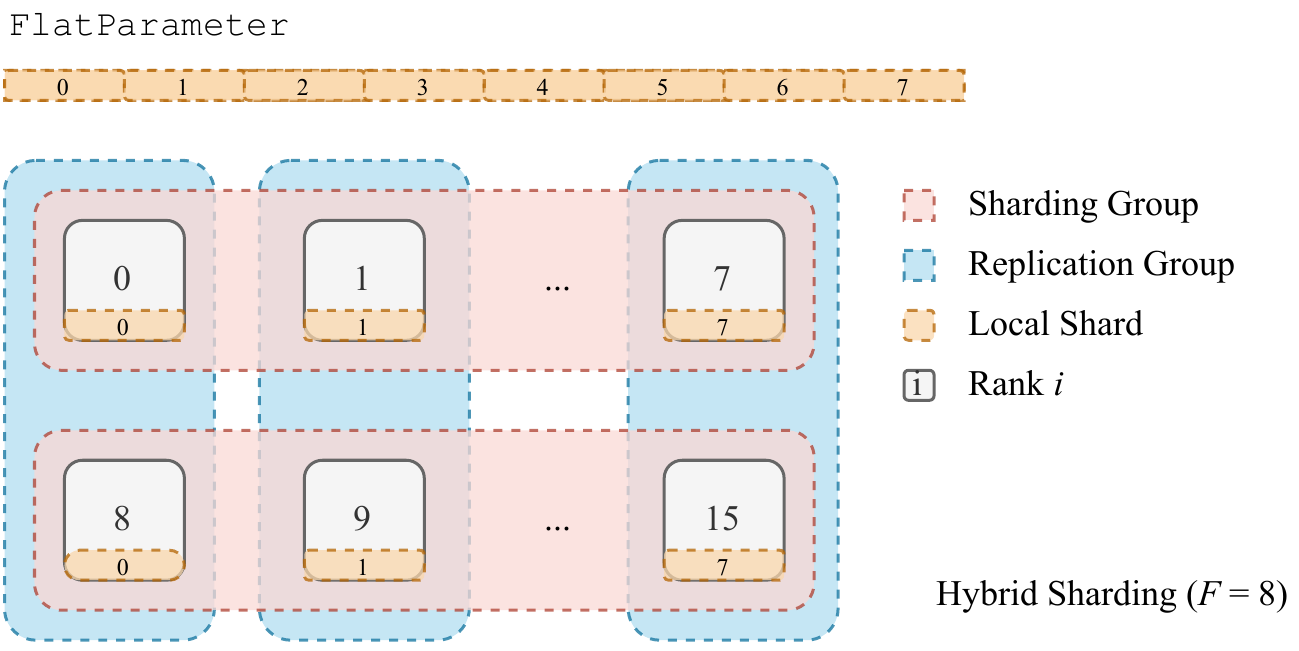
\includegraphics[width=\linewidth,height=0.42\textheight,keepaspectratio]{images/distributed-training/fsdp_fig4_hybrid_sharding.png}\\[0.2em]
      {\scriptsize Hybrid sharding on 16 GPUs: 2 sharding groups (rows) and 8 replication groups (columns), sharding factor $F = 8$. Zhao et al., \href{https://arxiv.org/abs/2304.11277v2}{arXiv:2304.11277v2}, Figure 4.}
  \end{columns}
  \vspace{0.3em}
  \begin{itemize}\footnotesize
    \item[\textcolor{red}{$\blacktriangleright$}] Hybrid sharding is the right default the moment a job spans more than one node and the model \emph{does} fit within one node's aggregate memory: it converts the $3\Psi$ inter-node bill back into $2\Psi$.
  \end{itemize}
\end{frame}

\begin{frame}[allowframebreaks]{FSDP1, FSDP2, and Choosing Between DDP and Sharding}
  \begin{itemize}\itemsep0.35em
    \item[\textcolor{red}{$\blacktriangleright$}] \textbf{FSDP1} (\texttt{FullyShardedDataParallel}) flattens and concatenates each unit's parameters into a single \texttt{FlatParameter}, then chunks it. Efficient, but the flattening hides the original tensors, which complicates frozen parameters, mixed dtypes, and state dicts.
    \item[\textcolor{red}{$\blacktriangleright$}] \textbf{FSDP2} (\texttt{fully\_shard}) shards each parameter individually on dimension 0 as a \texttt{DTensor}. Same throughput, but sharded state dicts need no all-gather, frozen parameters just work, and --- most importantly --- it \textbf{composes} with tensor, pipeline, and expert parallelism instead of needing special-case glue. FSDP1 is deprecated; new code should use \texttt{fully\_shard}.
    \item[\textcolor{red}{$\blacktriangleright$}] \textbf{When to prefer sharding over DDP:}
      \begin{itemize}\itemsep0.2em\footnotesize
        \item Model states do not fit on one device $\Rightarrow$ you have no choice: ZeRO-3 / \texttt{FULL\_SHARD}.
        \item They fit but leave almost no room $\Rightarrow$ ZeRO-2 / \texttt{SHARD\_GRAD\_OP} buys batch size at no extra communication.
        \item They fit comfortably and the interconnect is slow $\Rightarrow$ stay on DDP; sharding would add traffic you do not need.
      \end{itemize}
    \item[\textcolor{red}{$\blacktriangleright$}] \textbf{The limit of the whole family:} sharding still requires every rank to \emph{materialise} one full layer at a time. When a single layer's weights no longer fit on one GPU, no amount of data-parallel sharding helps --- and that is where tensor parallelism starts.
  \end{itemize}
\end{frame}
